\documentclass{article}
\usepackage{spconf,amsmath,graphicx}
\usepackage{lineno,hyperref}

\usepackage{amssymb,amsmath,graphicx,color,makecell,soul,booktabs,lipsum,dsfont,bbold}
\usepackage{mathrsfs}  
\usepackage{mathtools}
\usepackage[normalem]{ulem}
\DeclarePairedDelimiter\ceil{\lceil}{\rceil}
\DeclarePairedDelimiter\floor{\lfloor}{\rfloor}
\newcommand{\blockNs}{
 \begin{matrix}N & \cdots & N\end{matrix}}
 \newcommand{\blockOs}{
 \begin{matrix}0 & \cdots & 0\end{matrix}}
\newcommand{\blockN}[1]{
  \underbrace{\begin{matrix}N & \cdots & N\end{matrix}}_{#1}}
  \newcommand{\blockO}[1]{
  \underbrace{\begin{matrix}0 & \cdots & 0\end{matrix}}_{#1}}
\usepackage{soul}
\usepackage{xfrac}
\usepackage[utf8]{inputenc}
\DeclareMathOperator*{\argmax}{arg\,max}
\DeclareMathOperator*{\argmin}{arg\,min}
%\usepackage{caption}
\usepackage{float}
\usepackage{mwe}
% \usepackage{subcaption}
\usepackage[caption=false]{subfig}
\usepackage[utf8]{inputenc}
\usepackage[english]{babel}
 
\usepackage{amsthm}

\newtheorem*{remark}{Remark}

\def\lf{\left\lfloor}   
\def\rf{\right\rfloor}

\usepackage[english]{babel}
\usepackage{glossaries}

% Title.
% ------
\title{Artificial Intelligence for Defence \\in an EQF6 Training and Education Program,\\ from the Design to the Execution}

\name{TT$^{\star}$, YY$^{\dagger}$ ZZ$^{\dagger \ddagger}$}

\address{$^{\star}$ Univ. Bordeaux, Bordeaux INP, CNRS, FRANCE	\\ $^{\dagger}$ XX\\
 $^{\ddagger}$ YY}

\begin{document}

\maketitle
\begin{abstract}
In this paper, we present the main steps of the methodology we followed to design and prototype a module dedicated to artificial intelligence (AI) for defence for EQF-6 students. Based on a top-down approach for the design taking into account the market needs and some types of pedagogical activities, this module combines seasonal schools, invited speakers coming from the local ecosystems sharing their experience with AI and project based learning. It corresponds to 5 ECTS credits. Finally, a part of this module can be done in a hybrid way. 
\end{abstract}
%
\begin{keywords}
Artificial intelligence, Defence, Invited speakers, project based learning
\end{keywords}

\section{Introduction}
 Started in 2020, the ASSETS+ project, which stands for "Alliance for Strategic Skills addressing Emerging Technologies in Defence"  is an ERASMUS+ European project\footnote{More particularly, the project type is an Erasmus+ Sector Skills Alliance for implementing a new strategic approach (Blueprint) to sectoral cooperation on skills} the purpose of which is to build a sustainable human resources supply chain for the European defence industry, in order to boost innovation by both attracting highly-skilled young workers and upskilling its employees.  The consortium gathers 7 companies from the defence industry, 9 higher education institutes (HEI), 4 vocational educational and training (VET) providers, sectoral organizations and research centres, from 8 different countries. The goals of the projects are numerous:
1. analysing the emerging trends in technologies and deducing the skills that are required by now in many fields such as robotics, autonomous systems, artificial intelligence (AI), cybersecurity, and C4ISTAR (command, control, communications, computers, information-intelligence, surveillance, targeting acquisition and reconnaissance). 2. Designing and prototyping new education and training programmes for defence at three different levels from EQF4/5 to EQF 7\footnote{In the European Qualifications Framework (EQF), Level 4/5 corresponds to higher national diplomas while EQF 6 is related to the Bachelor degree. Finally, EQF 7 includes the Master’s degrees} either for students or for workers for upskilling or reskilling. The mid-term goal is to attract highly-skilled students in the domain, train the future defence sector workers and upskill the employees already working in the sector.  To this end, a common methodology has to be followed to get an easy qualification in terms of ECTS credits\footnote{European Skills/Competences, Qualifications and Occupations}, EQF level and ESCO taxonomy\footnote{European Skills/Competences, Qualifications and Occupations (ESCO).}
3. Developing a European Defence Qualification System covering pedagogical and technical aspects while complying with education requirements and industrial needs.

It should be noted that ASSETs+ is a member of the Pact for Skills, which is a shared engagement model for skills development in Europe. Through the Pact for Skills, the European Commission is bringing together companies, workers, national, regional and local authorities, social partners, cross-industry and sectoral organizations, education and training providers, chambers of commerce and employment services in order to create a culture of lifelong learning at work.

In this paper, we propose to present one of the modules that have been designed and prototyped for EQF-6 students. It deals with AI for defence and combines different types of pedagogical activities: seasonal schools with invited speakers coming from the local eco-system and project-based learning.
The remainder of this paper is organized as follows: In section 2, the design methodology is described. In section 3, details about the module are given. Finally, in section 4, feedbacks and testimonies are provided.
\section{Design methodology used for the module}
\begin{figure}[htb]
    \centering
    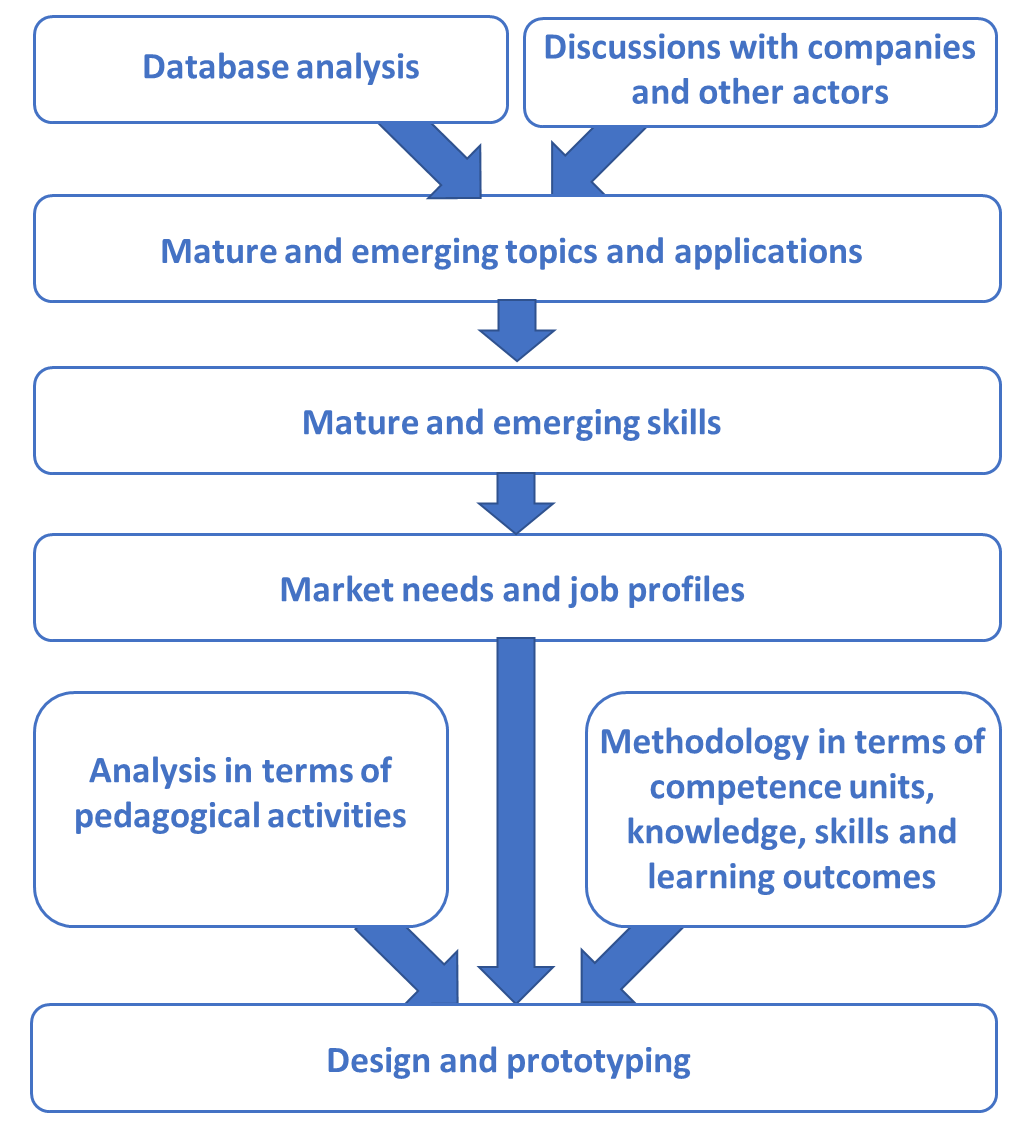
\includegraphics[width=\columnwidth]{timeflow_assetseqf6.png}
    \caption{Timeline of the design and prototyping of the EQF training and education program}
\end{figure}
\subsection{Some concerns about pedagogical activities}
The first step of the methodology we followed was to identify the pedagogical approaches that could be well suited to develop defence-related skills needed across Europe. To this end, some workshops were organized to better know each other and present some pedagogical approaches already implemented. See for instance [ref to be added]. When starting the design, our motivations were numerous: taking into account the market needs, improving the synergies between academia and industry in the domain, developing pedagogical activities encouraging students to respect a work ethic, to develop an entrepreneurial spirit, to foster creativity and innovation and to develop intercultural awareness and individual responsibility. 
Indeed, our purpose is to develop a skill-based approach where the concepts of knowledge and competency must be clearly distinguished. Thus, knowledge corresponds to the learning foundation while the competency is a set of general and specific knowledge, know-how, and life skills used to solve a problem. Students must hence be embedded in an environment in which they have to learn how to use and apply knowledge. If some lectures remain as one of the pillars in training programs, additional pedagogical activities must be added in order to introduce the context and to present the applications as well as the issues related to defence sectors so that the students can have a more concrete vision of the topic. 
To this end, seminars in which different actors of the domain coming from the industry or clusters was one of the suggestions we kept in mind. Project-based and problem-solving activities as well as seasonal schools could also be deployed.  
\subsection{Guidelines to be followed}
We follow a guideline to design the training program in compliance with European Qualification Standards, the European Qualifications Framework (EQF), the ECTS and ESCO taxonomy.

The approach we followed consists in designing competence units (CUs), corresponding to a set of modules of qualifications, consisting of a coherent set of knowledge and skills. The latter are written in terms of learning outcomes which express what the students know, understand and are able to do at the end of a learning process. The way these learning outcomes are written must be in line with what is expected at the EQF level. In other words, it must be written with specific descriptors defined in terms of knowledge, skills and autonomy-responsibility. Thus, for EQF 6 level, the students must show advanced knowledge in the field. This involves a critical understanding of the theories and the principles that have been presented. In terms of what is called cognitive and practical skills\footnote{peut-etre ajouter ce que l'on entend par la}, the students have to demonstrate their interest for innovation and their ability to solve complex problems. Finally, for what concerns responsibility and autonomy, the students are expected to manage complex technical or professional activities or projects, taking responsibility for decision-making in unpredictable work or study contexts. In addition, they should be also able to take responsibility for managing professional development of individuals and groups. 
\subsection{Application of this methodology for a module dedicated to AI for defence}
In terms of knowledge, the objective is to create a module so that the students can have 
advanced knowledge and critical understanding of the theory, principles and applicability of: 
\begin{enumerate}
    \item Machine Learning (ML) overview,
    \item Model training and evaluation 
\item Core ML algorithms 
\item 
ML issues and set of practices making it possible to deploy and maintain ML models in production reliably and efficiently (MLops)
\end{enumerate}
In terms of skills, this means that the trainees should be able to 
\begin{enumerate}
    \item Prepare datasets for training, \textit{i.e.} be able to gather, analyse and pre-process real-world data to train ML models upon. 
\item Build ML models on various data types, \textit{i.e.} be able to train models that will be able to infer useful results from training data. 
\item Use standard Python libraries for ML, \textit{i.e.} be able to know and use efficiently the essential tools of the Python ML landscape. 
\item Understand the benefits and limits of ML approaches, \textit{i.e.} be able to choose between a ML-based approach and a traditional, rule-based one depending on the project context and objective. 
\item Apply ML wisely, in accordance with ethical rules, \textit{i.e.} be able to understand and take into account the potential social and societal impacts of AI. 
\end{enumerate}
From a design point of view, this led to a module with 42 hours of contact hours.

Remark: It could be recommended to have other competence units in the whole training program: one dedicated to mathematics for Data Science dealing with introduction and review of probability and statistics, elements from information theory, review of linear algebra 
and optimization methods.  Another one should be related to programming in which 
programming environments, algorithmic structures, data structures and object-oriented programming are addressed. The last one can be dedicated to signal processing for ML in which the students learn some concepts dealing with signal processing, image processing, Markov decision processes and signal and image processing for ML.\\In the following, let us focus our attention on the 3 ECTS-module dedicated to ML. it addresses different concepts related to machine learning, from a general introduction to its application in the defence sector through state-of-the-art techniques and tools. The course is composed of three seasonal schools lasting between 2 and 3 days. During them, invited speakers coming from the AI for defence ecosystem put in perspective the topics at hand.
A project-based learning activity acts as a fil conducteur for students to apply their new knowledge and skills. 

 


\section{From the design to the prototyping}

\begin{figure}[ht]
    \centering
    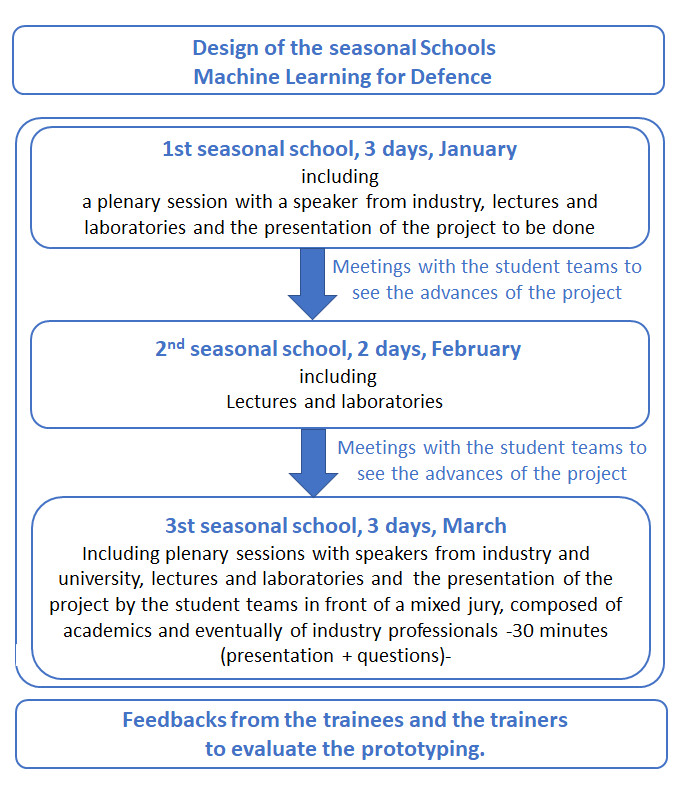
\includegraphics[width = \columnwidth]{assetsscpbl.png}
    \caption{Timeline of the proj}
e\end{figure}

\subsection{Project: Cyber-security as a Use Case}
As a use case, the participants were involved in the design of ML and DL models to detect malware in Android apps. They were provided with a dataset coming from static and dynamic analysis of benign and malware apps. The dataset was sufficiently large to be split into two parts: one for the training and one for the  test. 
The 


speaking of the invited speakers (academic and industrials)\\
giving the topic of the project and the reason why we decided to use this project\\
speaking of the social program\\
speaking of the obstacles we face\\
\section{Feedbacks}
\section{Conclusions and perspectives}


\newpage
%\bibliographystyle{IEEEbib}
%\bibliography{ref}
\end{document}